\documentclass{beamer}
%pacchetti
\usepackage[T1]{fontenc}
\usepackage[utf8]{inputenc}
\usepackage{graphicx}
\usepackage[italian]{babel}
\usepackage{mathrsfs}
\usepackage{booktabs}
\usepackage{amsmath}
\usepackage{amsfonts}
\usepackage{amssymb}
\usepackage{amsbsy}
\usepackage{amsthm}
\usepackage{enumerate}
\usepackage{quoting}
\quotingsetup{font=small}
\usepackage{diagbox}
\usepackage{graphicx}
\usepackage{setspace}
\usepackage{float}
\usepackage{version}
\usepackage{multicol}
\usepackage{beamerfoils}

\usepackage[none]{hyphenat} %avoid hyphenation
\usepackage{xcolor} %to uset \textcolor
\usepackage{bbm} %funzione indicatrice
% end pacchetti

\usetheme[bgphoto]{polimi}

% Full instructions available at:
% https://github.com/elauksap/beamerthemepolimi

% Set custom font (requires to compile with XeLaTeX).
\usepackage{ifxetex}
\ifxetex
\usepackage{fontspec}
\setsansfont[Scale=0.9]{Arial}
\fi

\usepackage{lipsum}


\newcommand\mynum[1]{%
	\usebeamercolor{enumerate item}%
	\tikzset{beameritem/.style={circle,inner sep=0,minimum size=2ex,text=enumerate item.bg,fill=enumerate item.fg,font=\footnotesize}}%
	\tikz[baseline=(n.base)]\node(n)[beameritem]{#1};%
}


\title{Coupled Markov chains with applications to Approximate Bayesian Computation for model based clustering}
%\subtitle{Subtitle}
\author{E. Bertoni, M. Caldarini, F. Di Filippo, G. Gabrielli, E. Musiari}
\date{10 January 2022}


%Cose da fare

% Mettere biografia
% Mettere \pause e colori
% Sistemare il titolo e layout

\begin{document}

\begin{frame}
\maketitle
\end{frame}

\begin{section}{Introduction}

	\begin{frame}
		\frametitle{A complex problem}

 		\begin{minipage}{0.45\textwidth}
 			\begin{center}
 				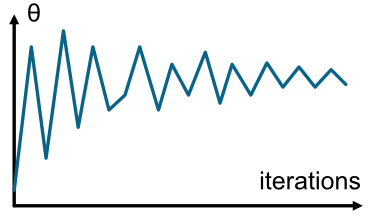
\includegraphics{img/markov_singola}
 			\end{center}
 		\end{minipage}
 		\hfill
 	 	\begin{minipage}{0.45\textwidth}
 	 		\begin{center}
 	 		%	\only<2>{
 	 				% 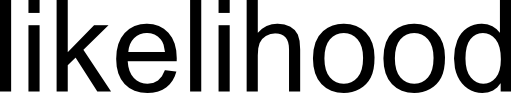
\includegraphics{img/likelihood} %}
 	 		%	\only<3,4,5>{
 	 				
\includegraphics{img/likelihood_na} %}
 	 		\end{center}
 		\end{minipage}
 		
 		\vspace{0.5cm}
 		
 	%	\only<4,5>{
 			\begin{minipage}{0.45\textwidth}
 			\begin{center}
 				$\Downarrow$

 				\textbf{Unbiased Markov chain Monte Carlo methods with couplings}
 			\end{center}
 		\end{minipage} %}
 		\hfill
 	%	\only<5>{
 	\begin{minipage}{0.45\textwidth}
 			\begin{center}
 				$\Downarrow$
 				
 				 \textbf{Approximate Bayesian Computation}
 			\end{center}
 		\end{minipage} %}
 	 	
 	 	\vspace{0.2cm}
 	 	
 	 %	\only<4,5>{
 	 		\begin{minipage}{0.45\textwidth}
 	 		\begin{center}
 	 			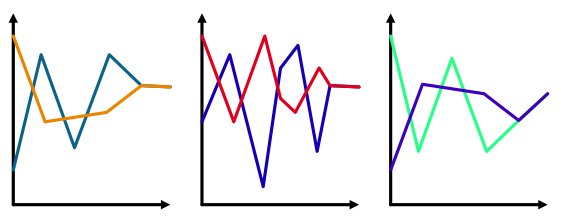
\includegraphics{img/markov_coupled_parallel}
 	 		\end{center}
 	 	\end{minipage}%}
 	 	\hfill
 	 	\begin{minipage}{0.45\textwidth}

 	 	\end{minipage}
 	 	
 	 	
 	 	
	\end{frame}

\end{section}



\begin{section}{Unbiased Markov chain Monte Carlo methods with couplings}
	\begin{frame}[plain]{}
		\sectionpage
	\end{frame}
	
	\begin{frame}
		\frametitle{Time-averaged estimator}
		\begin{enumerate}
			\item draw $X_0$ and $Y_0$ from an initial distribution $\pi_0$ and draw $X_1 \sim P(X_0, \cdot)$;
			\item set $t=1$: while $t<\max\{m,\tau\}$ and:
			\begin{itemize}
				\item[a] draw $(X_{t+1}, Y_t)\sim \bar P \{(X_t, Y_{t-1}), \cdot \}$; 
				\item[b] set $t \leftarrow t+1$;
			\end{itemize}
			\item compute the time-averaged estimator:
			\footnotesize{	 	$$
				H_{k:m}(X,Y)
				= \frac{1}{m-k+1}\sum_{l=k}^{m}h(X_l) 
				+ \sum_{l=k+1}^{\tau -1}\min(1, \frac{l-k}{m-k+1})\{h(X_l)-h(Y_{l-1})\} .
				$$
			}
		\end{enumerate}
	\end{frame}
	
	\begin{frame} 	
		\frametitle{Metropolis--Hasting algorithm for a coupled kernel}
		Metropolis--Hasting algorithm allow us to calculate the coupled kernel $\bar P \{(X_t, Y_{t-1}), \cdot \}$:

			\begin{enumerate}
				\item sample $(X^\star, Y^\star) | (X_t, Y_{t-1})$ from a maximal coupling of $q(X_t, \cdot)$ and $q(Y_{t-1}, \cdot)$;
				\item sample $U \sim \mathcal{U}([0,1])$;
				\item if
				$$ U
				\leq \min\bigg \{
				1,
				\frac{ \pi(X^\star)q(X^\star,X_t)}{
					\pi(X_t)q(X_t, X^\star)}
				\bigg \}
				$$
				then $X_{t+1} = X^\star$; otherwise $X_t = X_{t-1}$;
				\item if
				$$ U
				\leq \min\bigg \{ 
				1,
				\frac{ \pi(Y^\star)q(Y^\star,Y_t)}{
					\pi(Y_t)q(Y_t, Y^\star)}
				\bigg \}
				$$
				then $Y_{t+1} = Y^\star$; otherwise $Y_t = Y_{t-1}$.
				
			\end{enumerate}
	\end{frame}


	\begin{frame}
		\frametitle{Maximal coupling}
		The algorithm:\\
		
		Set $p = \mathcal{N}(X_{t-1},1)$ and $q = \mathcal{N}(Y_{t-1},1)$,
		\begin{enumerate}
			\item sample $X_t \sim p$;
			\item sample $W|X_t \sim \mathcal{U}\{[0,p(X_t)]\}$;
			\item if $W\leq q(X_t)$ then output $(X_t,X_t)$, otherwise:
			\begin{enumerate}
				\item sample $Y_t \sim q$;
				\item sample $W^\star | Y_t \sim \mathcal{U}\{[0, q(Y_t)]\}$ 
				until $W^\star > p(Y_t)$ and output $(X_t,Y_t)$.
			\end{enumerate}
		\end{enumerate}
	\end{frame}

	\begin{frame}
		\frametitle{Study case}
		
		\begin{block}{Model}
			\begin{center}
				$ Y_i | \mu \overset{iid}{\sim} \mathcal{N}(\mu, \sigma_{obs} ^2) $\\
				
				\vspace{0.3cm}
				
				$ \mu  \sim \mathcal{N}(\mu_0, \sigma_0^2)$
				
				$\mu_0 = 38, \quad \sigma^2_0 = 4$
			\end{center}
		\end{block}
		
		\begin{block}{Dataset}
			1000 samples generated from a Gaussian distribution:
			\begin{center}
				$
				Y_{obs} \sim \mathcal{N}(\mu_{obs}, \sigma_{obs} ^2)
				$
				
				$
				\mu_{obs} = 43, \quad
				\sigma_{obs} ^2 = 5
				$
			\end{center}
		\end{block}
	\end{frame}

	\begin{frame}
		\frametitle{Implementation and parallelization}
	\end{frame}

	\begin{frame}
		\frametitle{Results}
		
		$\mathcal{N}(\mu_n, \sigma^2_n)$
		$\mu_n = 
		y= tfd.Normal(
		1/(1/sigma0*2 + n/sigma_obs2)(mu0/sigma0*2 + (np.sum(y)/sigma_obs2)),
		1/(1/sigma02 + n/sigma_obs*2)
		)   
		$

		\begin{itemize}
			\item posterior
			\item risultato del time averaged
			\item grafico catene che si incontrano
			\item istogramma dei samplings (sotto alla posterior)
		\end{itemize}
	\end{frame}
	
\end{section}


\begin{section}{Approximate Bayesian Computation}
	
	\begin{frame}[plain]{}
		\sectionpage
	\end{frame}
	
	%%%% (dire quale summary statistica usata, quale distanza usata, quale kernel)
\begin{frame}{ABC rejection sampling algorithm}
	NO, UTILIZZARE ALGORITMO DI PAGINA 103
	\only<1> {
		\emph{Inputs:}
		\begin{itemize}
			\item a target posterior density $\pi(\theta | y_{obs}) \propto p(y_{obs}|\theta) \pi(\theta)$, consisting of a prior distribution $\pi(\theta)$ and a procedure of generating data under the model $p(y_{obs}|\theta)$;
			\item a proposal density $g(\theta)$, with $g(\theta)\textgreater 0 $ if $\pi(\theta | y_{obs}) \textgreater 0$;
			\item an integer $N \textgreater0$;
			\item a kernel function $K_h(u)$ and a scale parameter $h > 0$;
			\item a low dimensional vector of summary statistics $s=S(y)$.
		\end{itemize}
	}
	\only<2> {
		\emph{Sampling} for $i= 1,..., N$:
		\begin{enumerate}
			\item generate $\theta ^ {(i)} \sim g(\theta)$ from sampling density $g$;
			\item generate $ y \sim p(y|\theta ^ {(i)})$ from the likelihood;
			\item compute summary statistic $s = S(y)$;
			\item accept $\theta ^ {(i)}$ with probability $\frac{K_h(\parallel s-s_{obs}\parallel)   \pi(\theta ^ {(i)})}{K g(\theta ^ {(i)})}$, where $K \geq K_h(0)\max_{\theta}{\frac{\pi(\theta)}{g(\theta)}}$; else go to 1.
		\end{enumerate}
		
		\emph{Output:}
		\begin{itemize}
			\item a set of parameter vectors $\theta ^ {(1)},..., \theta ^ {(N)} \sim \pi_{ABC}(\theta |S_{obs})$.
		\end{itemize}
	}
	\end{frame}
	
	\begin{frame}{}
		summary statistics: media
		distanza: norma (modulo della differenza)   (mahalanobis nel caso multivariato)
		kernel: 1/(np.sqrt(2*math.pi))np.exp(-1/2*u*2)
		% parlare di abc in caso univariato -> le nostre scelte come summary statistics, distanza, kernel
	\end{frame}

	\begin{frame}
		\frametitle{Study case}
		
		\begin{block}{Model}
			\begin{center}
				$ Y_i | \mu \overset{iid}{\sim} \mathcal{N}(\mu, \sigma_{obs} ^2) $\\
				
				\vspace{0.3cm}
				
				$ \mu  \sim \mathcal{N}(\mu_0, \sigma_0^2)$
				
				$\mu_0 = 38, \quad \sigma^2_0 = 4$
			\end{center}
		\end{block}
		
		\begin{block}{Dataset}
			1000 samples generated from a Gaussian distribution:
			\begin{center}
				$
				Y_{obs} \sim \mathcal{N}(\mu_{obs}, \sigma_{obs} ^2)
				$
				
				$
				\mu_{obs} = 43, \quad
				\sigma_{obs} ^2 = 5
				$
			\end{center}
		\end{block}
	\end{frame}
	
	\begin{frame}{}
		% grafici per un esempio univariato con summary mean -> e uno con quantili? (funzionava?)
	\end{frame}
	
	\begin{frame}{}
		%
	\end{frame}


\end{section}






\begin{section}{Conclusions}
	
    \begin{frame}[plain]{}
		\sectionpage
	\end{frame}

	\begin{frame}{Next steps}
	
		The next step will be the conclusion of the \textbf{separate multivariate implementation} of both solution to be tested on simulated data and the \textbf{parallelized multivariate implementation}.
		
		\vspace{0.5 cm}
		Further steps will be testing on more complex data.
	\end{frame}

	\begin{frame}{Bibliography}
		\nocite{*}
		\bibliographystyle{unsrt}
		\tiny{ \bibliography{refs_MCMC,refs_ABC} }

	
%				\begin{minipage}[t]{0.4\textwidth}
%			\footnotesize {Unbiased Markov chain Monte Carlo methods with couplings:}
%			\tiny { \bibliography{refs_MCMC} }
%		\end{minipage}
%		\hfill
%		\begin{minipage}[t]{0.4\textwidth}
%			\footnotesize {Approximate Bayesian computation:}
%			\tiny { \bibliography{refs_ABC} }
%		\end{minipage}

	\end{frame}
\end{section}

\end{document}
